%HW04.tex
%Fourth Homework -- Math 629 
%
%  The percent sign is a comment character
%
%%%%%%%%%%%%%%%%%%%%%%%%%%%%%%%%%%%%%%%%%%%%%%%%%%%%%%%%%%%%%%%%%%%%%%%%%%%%%%%%%%
%
%   Look these up on line.  The first sets the type of document, and the next are for mathematics symbols, graphics and color
%
\documentclass[12pt]{article}
\usepackage{amssymb,amsmath}
\usepackage{graphicx}
\usepackage[usenames,dvipsnames,svgnames,table]{xcolor}
\usepackage{multirow}   % This is for more control over tables
%%%%%%%%%%%%%%%%%%%%%%%%%%%%%%%%  Layout     %%%%%%%%%%%%%%%%%%%%%%%%%%%%%%%%%%%%%%
\usepackage{vmargin}
\setpapersize{USletter}
\setmargrb{2cm}{1cm}{2cm}{1cm} % --- sets all four margins LTRB


%%%%%%%%%%%%%%%%%%%%%%%%%%%%%%%%%%%%%%%%%%%%%%%%%%%%%%%%%%%%%%%%%%%%%%%%%%%%%%%%%
\begin{document}
\LARGE 
\noindent
{\color{Maroon}History of Mathematics \hfill Math 629}\vspace{2pt}\\
\large
Fourth Homework: \hfill 7 February 2024\\
Due Monday 12 February 2024.
\normalsize\vspace{10pt}

To hand in: We are using Gradescope for homework submission.


\begin{enumerate}

\item  Do exercises 5.4.5 and 5.4.6 in Stillwell.
  The webpage includes some discussion of hyperbolic functions that you will need.
  (I assume that you know everything about the sine and cosine functions.)

\item   Rational triangles.  Do the exercises in Stillwell: 5.6.1,  5.6.2,  5.6.3,  and  5.6.4.


\item   Prove the following generalization of Pythagoras' Theorem:
  Consider a triangle $ABC$. Mark points $D$ and $E$ on the side $BC$ so that the angles $BAC$, $ADB$, and $AEC$ are congruent
  as shown below.
  Prove that $(AB)^2 + (AC)^2 = BC(BD + EC)$.  While the result does not need that the angle $BAC$ is obtuse, it helps if we draw it that
  way (as shown below).
  It helps to use proportions and similar triangles.

  \begin{picture}(200,230)
      \put(0,0){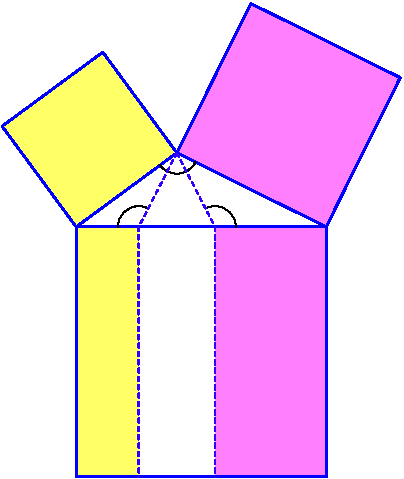
\includegraphics{NewPythagoras}}
      \put(80,168){$A$}
      \put(23,118){$B$}       \put(162,118){$C$}
      \put(68,109){$D$}       \put( 91,109){$E$}
  \end{picture}
  
\end{enumerate}

\end{document}
%%%%%%%%%%%%%%%%%%%%%%%%%%%%%%%%%%%%%%%%%%%%%%%%%%%%%%%%%%%%%%%%%%%%%%%%%%%%%%%%%
